%% 
%% Copyright 2007-2020 Elsevier Ltd
%% 
%% This file is part of the 'Elsarticle Bundle'.
%% ---------------------------------------------
%% 
%% It may be distributed under the conditions of the LaTeX Project Public
%% License, either version 1.2 of this license or (at your option) any
%% later version.  The latest version of this license is in
%%    http://www.latex-project.org/lppl.txt
%% and version 1.2 or later is part of all distributions of LaTeX
%% version 1999/12/01 or later.
%% 
%% The list of all files belonging to the 'Elsarticle Bundle' is
%% given in the file `manifest.txt'.
%% 
%% Template article for Elsevier's document class `elsarticle'
%% with harvard style bibliographic references

\documentclass[preprint,12pt,authoryear]{elsarticle}
%\documentclass[10pt,final,journal,compsoc,a4paper]{IEEEtran}
%% Use the option review to obtain double line spacing
%% \documentclass[authoryear,preprint,review,12pt]{elsarticle}

%% Use the options 1p,twocolumn; 3p; 3p,twocolumn; 5p; or 5p,twocolumn
%% for a journal layout:
%% \documentclass[final,1p,times,authoryear]{elsarticle}
%% \documentclass[final,1p,times,twocolumn,authoryear]{elsarticle}
%% \documentclass[final,3p,times,authoryear]{elsarticle}
%% \documentclass[final,3p,times,twocolumn,authoryear]{elsarticle}
%% \documentclass[final,5p,times,authoryear]{elsarticle}
%% \documentclass[final,5p,times,twocolumn,authoryear]{elsarticle}

%% For including figures, graphicx.sty has been loaded in
%% elsarticle.cls. If you prefer to use the old commands
%% please give \usepackage{epsfig}

%% The amssymb package provides various useful mathematical symbols
\usepackage{amssymb}
\usepackage{pgf-pie}
\usepackage{calc}
\usepackage{graphicx}
\usepackage{float}
\usepackage{anyfontsize}
\usepackage{pgfplots}

%% The amsthm package provides extended theorem environments
%% \usepackage{amsthm}

%% The lineno packages adds line numbers. Start line numbering with
%% \begin{linenumbers}, end it with \end{linenumbers}. Or switch it on
%% for the whole article with \linenumbers.


\addbibresource{references.bib} %Imports bibliography file


\journal{Energy and Buildings}

\begin{document}

\begin{frontmatter}

%% Title, authors and addresses

%% use the tnoteref command within \title for footnotes;
%% use the tnotetext command for theassociated footnote;
%% use the fnref command within \author or \affiliation for footnotes;
%% use the fntext command for theassociated footnote;
%% use the corref command within \author for corresponding author footnotes;
%% use the cortext command for theassociated footnote;
%% use the ead command for the email address,
%% and the form \ead[url] for the home page:
%% \title{Title\tnoteref{label1}}
%% \tnotetext[label1]{}
%% \author{Name\corref{cor1}\fnref{label2}}
%% \ead{email address}
%% \ead[url]{home page}
%% \fntext[label2]{}
%% \cortext[cor1]{}
%% \affiliation{organization={},
%%            addressline={}, 
%%            city={},
%%            postcode={}, 
%%            state={},
%%            country={}}
%% \fntext[label3]{}

\title{TIMES Ireland Model: Residential Sector}

\author[inst1,inst2]{Jason Mc Guire\footnote{Contact: j.mcguire@ucc.ie}}

\affiliation[inst1]{organization={Energy Policy and Modelling Group, MaREI Centre},%Department and Organization
            addressline={Environmental Research Institute}, 
            city={Cork},
            country={Ireland}}
            
\affiliation[inst2]{organization={School of Engineering},%Department and Organization
            addressline={University College Cork}, 
            city={Cork},
            country={Ireland}}


\author[inst1,inst2]{Fionn Rogan}
\author[inst1,inst2]{Olexandr Balyk}
\author[inst1,inst2]{Hannah Daly}
\author[inst1,inst2]{ \& Brian Ó Gallachóir}

\begin{abstract}
%% Text of abstract

Write after paper is completed %Ireland's residential sector has particularly underachieved in previous climate targets.  Located on the peripherals of Europe, with a high share of low thermal efficient detached dwellings with carbon intensive heating fuels, provides some distinctive barriers to decarbonising Ireland's residential sector. The disadvantageous starting position has impeded residential decarbonisation progress thus far. \par
%Energy system optimization models (ESOMs) have been used extensively to inform pathways in addressing long-term energy challenges which provides insights to decision makers on issues related to climate and energy policy. \par
%The TIMES-Ireland Model (TIM) is a newly developed optimisation model of the Irish energy system, which calculates the  cost-optimal decarbonisation pathway to meet future energy service demands while achieving Ireland's legally binding 2030 and 2050 climate targets.
 
\end{abstract}

%%Graphical abstract
%%\begin{graphicalabstract}
%%\includegraphics{grabs}
%%\end{graphicalabstract}

%%Research highlights
%%\begin{highlights}
%%\item Research highlight 1
%%\item Research highlight 2
%%\end{highlights}

\begin{keyword}
%% keywords here, in the form: keyword \sep keyword
Energy systems optimisation model (ESOM) \sep The integrated MARKAL-EFOM system (TIMES) \sep Building decarbonisation \sep Model description \sep Residential energy transition
%% PACS codes here, in the form: \PACS code \sep code
%%\PACS 0000 \sep 1111
%% MSC codes here, in the form: \MSC code \sep code
%% or \MSC[2008] code \sep code (2000 is the default)
%% \MSC 0000 \sep 1111
\end{keyword}

\end{frontmatter}

%% \linenumbers

%% main text
\section{Introduction}
\label{sec:Introduction}
\subsection{Climate Targets}
\label{Intro:Climate Targerts}
\par % Paragraph 1 - Intro
Under the Climate Action and Low Carbon Development (Amendment) Act 2021, the Irish government has proposed legally binding national targets to reduce Greenhouse Gas (GHG) emissions by 51\% in 2030 compared to 2018. The Act also proposes a long-term target to achieve a climate neutral economy or ``net-zero" by 2050 \cite{2021Climate2021}. These targets accounts for all GHGs - both Emission Trading System (ETS) emissions and non-ETS emissions, and sets out to develop sectoral five year carbon budgets to aid progress of the forementioned long-term targets. 
\par The EU's first Nationally Determined Contribution (NDC) which had a 40\% GHG reduction target (first NDC), has increased to at least a 55\% GHG reduction target (updated NDC) by 2030 compared to 1990 levels \cite{SUBMISSIONSTATES}. Ireland's Climate Action Plan 2019 (CAP2019) which complies with EU's first NDC, from which Irelands 30\% Non-ETS GHG reduction target in 2030 compared to 2005 levels was derived  \cite{DepartmentofCommunicationsClimateActionandEnvironment2019Climate2019}. Climate Action Plan 2021 will have to be more ambitious than its predecessor, as it must at least reflect EU's updated NDC target. Assuming the share of contribution of ETS and Ireland's Non-ETS remains the same, Ireland's non-ETS GHG emission 2030 target would change from 30\% to 45\%. Overall Ireland's national 2030 target would be about 15\% more ambitious than the EU's updated NDC.
There are also renewable energy targets to consider for transport (RES-T), heat (RES-H) and electricity (RES-E) under renewable directive (EU) 2018/2001, and energy efficiency targets under (EU) 2018/2002. An overview of Ireland's climate targets are shown in Fig.\ref{fig:IrelandClimatetargets}. 

\begin{figure}[!htbp]
 \centering
 \includegraphics[scale=0.4]{Figures/Non-ETS-Share.png} 
 \caption{Overview of Ireland's 2030 Climate Targets}
 \label{fig:IrelandClimatetargets}
\end{figure}

Ireland is a unique EU member state, located on the peripherals of Europe, with a the second highest GDP per capita \cite{EurostatReal} (Higher GDP per capita translates to higher non-ETS reduction target), the largest proportion of agriculture GHG emissions at 34\% in 2018  \cite{EPA2020Irelands1990-2018}, and a high dependency on fossil fuel imports. Ireland has been afforded high non-ETS flexibility allowances under (EU) 2020/2126, to compensate for these barriers, but Ireland still has ambitious national climate targets. To put Ireland's climate targets in perspective Fig.\ref{fig:GHG2030AGR} compares different countries 2030 climate target with a 2018 base year and share of agriculture GHG emissions. Ireland has ambitious targets, despite distinct barriers. The Climate Change Advisory Council (CCAC) will rely of some modelling tools to provide insights and set sectoral five year carbon budgets.

\begin{figure}[!htbp]
 \centering
 \includegraphics[scale=0.5]{Figures/GHGtargetAGR1.png} 
 \caption{Most Ambitious 2030 GHG Targets}
 \label{fig:GHG2030AGR}
\end{figure}
 
\subsection{Energy System Optimisation Models}
\label{Intro:ESOM}
\par % Paragraph 2 - ESOM
A Energy System Optimisation Model (ESOM) can optimise the selection of a large number of dynamic variables to satisfy demand, while accounting for complex economic sectoral interconnections within each time period. The ESOM described in this paper is The Integrated MARKAL-EFOM System (TIMES) modelling framework, which has been developed and maintained by Energy Technology Systems Analysis Program (ETSAP) of the International Energy Agency (IEA). TIMES is a ``hybrid" ESOM, which combines high resolution ``bottom-up" technological detail and ``top-down" macroeconomic variables covering all energy sectors.
\par In addition to TIMES there are other ESOM frameworks available such as EnergyPLAN \cite{stergaard2015ReviewingSimulations}, MESSAGE \cite{Messner1995WorkingE}, Balmorel \cite{Wiese2018BalmorelModel}, TEMOA \cite{Hunter2013ModelingTemoa} and OSeMOYS \cite{Howells2011OSeMOSYS:Development.}. However the expertise among energy policy researchers in Ireland combined with the global network of ETSAP modellers, makes TIMES the preferred ESOM to explore Ireland's decarbonisation pathways. \par Previous versions of the Irish TIMES model were extracted from the Pan European TIMES model, and then updated with specific national data and assumptions. The previous Irish TIMES models were used to provide informative reports on Irish climate policy \cite{Gallachoir2012EPAModel,Deane2017Irish2,Gallachoir2020The3,Deane2013TechnicalIreland,IrishGovernment2017National2017}.  
While TIMES models can cover all the energy-related sectors, it can also be used to explore the residential sector in detail. Some studies focusing on the residential sector in TIMES include, Li who studied the preference for heating technology choice in UK \cite{Li2018IncorporatingModel}, Petrovic examined a new approached to represent residential heat pumps in Denmark \cite{Petrovic2016ResidentialSystem} and Aberg analysed the affect higher thermal efficiency in buildings has on co-production of electricity and district heating in Sweden \cite{Aberg2011OptimisationBuildings}. There has also been some studies residential sector in Ireland, using previous versions of Irish TIMES and now out-dated climate targets. Therefore, there is a need for a new TIMES model to be built specifically to explore Ireland's new 2030 and 2050 climate targets and sectoral five-year carbon budgets, the ``TIMES Ireland Model" (TIM) was built in 2021 to address this need \textbf{(SOURCE)}.

\subsection{Ireland: Residential Sector Background}
\label{Intro:IreRSDBack}

\par
Ireland’s distinctive decarbonisation pathway, is further separated from other EU member states when focusing on the residential sector. This is largely down to Ireland’s high reliance on fossil fuels, low building thermal efficiency, larger dwellings and rural settlement patterns. This is illustrated by the fact only 5.8\% of the population of Ireland were living in apartments in 2018, the lowest in EU-27 and well below the 25.3\% average \cite{EurostatDistributionSurveyilc_lvho01}, furthermore 71.4\% of the Irish population are deemed to be living in dwellings too large, where the EU-27 rate is 33\% \cite{EurostatShareSurveyilc_lvho50a}. The low thermal efficiency of Ireland's dwelling is discussed later in this section and highlighted in Fig.\ref{fig:BERAge}. Furthermore Irelands fossil fuel dependency is underlined by home heating oil accounting for the largest share of fuel usage in the residential sector at 37\% \cite{SustainableEnergyAuthorityofIreland2018EnergySector}, of which all is imported \cite{OCleirigh2020ENERGYReport}.

In the last 30 years, the extraction of indigenous peat has declined and consequently peat consumption has halved, in 2018 peat accounted for 12.3\% of residential GHG emissions. Residential coal GHG emissions has also declined to 6.9\% in 2018 \cite{EnergySEAI}. However, the decline in peat and coal has been offset by more significant growth in oil in the same period, where oil accounted for 34.8\% of residential GHG emissions in 2018 \cite{Howley2005ENERGY-RELATEDIreland}. Gas which is only available in some urban areas, accounted for 15.5\% of residential GHG emission in 2018 \cite{Howley2005ENERGY-RELATEDIreland}.  
In summary, the residential sector is highly reliant on fossil fuels as shown in Fig.\ref{fig:ResFuel}, consequently Ireland currently has the lowest renewable heat of  among EU member states, at only 6.3\% \cite{Eurostat2021ShareSourcesnrg_ind_ren}. 

\begin{figure}[!htbp]
 \centering
 \includegraphics[scale=0.5]{Figures/ResidentialFuelUsage.png}
 \caption{Historical Residential Fuel Consumption}
 \label{fig:ResFuel}
\end{figure}
% NOTE THE Y-AXIS IS NOT CORRECT - DATA FROM SEAI ENERGY DATA PORTAL 


The 2021 building regulations in 2021 require a 70\% reduction of CO2 emissions in new dwellings compared to 2005 \cite{DepartmentofHousingGov.ieBuildings}, but since the 2008 global financial crisis there has been a considerable slowdown in the growth of housing stock. According to Central Statistics Office (CSO) approx. 85\% of residential buildings are 2005 or older. The BER database, which represents half of the dwelling stock, highlights the affect of construction year on the expected energy consumption, as shown in Fig.\ref{fig:BERAge}. The BERs labels are categorised based on expected energy consumption, with A1 representing the lowest expected energy consumption ($\leq 74 kWh/m^2/year$) and G representing the highest expected energy consumption ($ >450 kWh/m^2/year$). The BERs are developed from the Energy Performance of Buildings Directive 2002/91/ EC, helps to better understand the housing stock. The BERs are required for new houses, rented houses, sold houses and renovated houses. 

\begin{figure}[!htbp]
 \centering
 \includegraphics[scale=0.5]{Figures/BERAge.png}
 \caption{Building Energy Rating by Age}
 \label{fig:BERAge}
\end{figure}

Theoretically G-rated BERs consume more energy and consequently have higher energy bills to maintain a comfortable internal temperature, but in reality G-rated dwellings have low internal temperatures, which results in higher excessive winter mortality \cite{Clinch2000HousingMortality}. BERs do not take account of actual usage based on occupancy behaviour or occupancy density, nor does it take account of the size of the dwelling. The BER labels do therefore leave a gap between actual consumption and expected consumption, I will explain how I approached this problem in the literature review. 

Fuel Poverty which is a major contributor to the high excessive winter deaths, is defined as when a \textit{``household spends 10\% or more of income to achieve adequate warmth"}. An Element Energy report claimed 28\% of Irish households were in fuel poverty in 2015  \cite{ElementEnergy2015Bottom-upIreland}. Fuel Allowance and the Household Benefits provides support to low income households to alleviate fuel poverty. These payments have been increased over time with a further increase made in Budget 2020, coinciding with the increase in the carbon tax \cite{,EuropeanUnion2020EUObservatory}. As Kerr's study finds an explicit link between fuel poverty and social welfare policy in Ireland \cite{,EuropeanUnion2020EUObservatory,Kerr2019PoliticsFrance} and O’Meara highlights the health issues associated with Fuel Poverty, which include increased risk of catastrophic cardiovascular or cerebrovascular events \cite{OMeara2016AIreland}. Ironically, it can be argued this places low income households deeply dependent on fossil fuels for health.

The United Nations Framework Convention on Climate Change (UNFCCC) GHG reporting rules, as per Decision 24/CP.19, states that 2006  Intergovernmental Panel on Climate Change (IPCC) guidelines are to be adhere to for national GHG reporting. Under these guidelines, Ireland’s residential sector accounted for 14.2\%of GHGs emissions in 2018 \cite{Howley2005ENERGY-RELATEDIreland}. Focusing on energy-related GHG emissions, the residential sector directly accounts for 24\% of GHG emissions. Fig. \ref{fig:Ireland2018GHG} shows the energy related GHG disaggregated between transport, heat and electricity. Where the residential sector is the direct source 47\% of heat and 30\% of electricity GHG emissions, the residential sector is therefore a pivotal sector in Ireland energy decarbonisation. 

\begin{figure}[!htbp]
    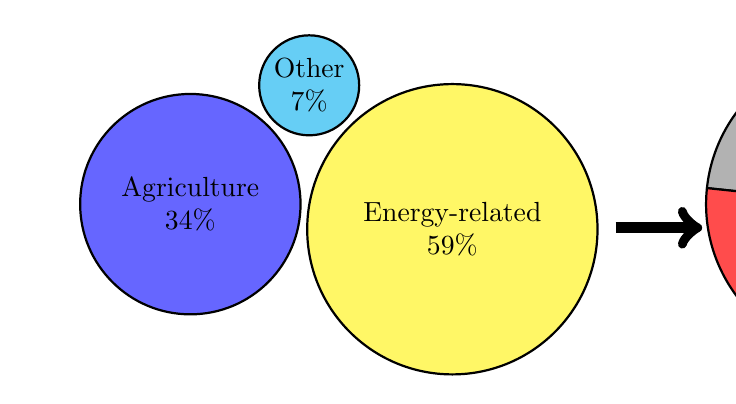
\begin{tikzpicture}[every node/.style={align=center}, pin distance=17mm]
    \pie[cloud,text=inside,radius = 2.4]{34/Agriculture,7/Other,59/Energy-related}
    \draw [->, line width=4pt] (5.4,-0.3) -- (6.5,-.3);
    \hspace{8.5cm}
    \pie[rotate =30,text=inside,radius=1.95,color={black!30,red!70,yellow!40}]{40/Transport,33/Heat,27/Electricity}
    \end{tikzpicture}
    \caption{Ireland 2018 GHG Share \cite{Howley2005ENERGY-RELATEDIreland}}
    \label{fig:Ireland2018GHG}
\end{figure}

\subsection{Residential Energy Services}
\label{Intro:EnergyServices}

Space heating is the largest residential energy service demand, accounted for 61.8\% of final energy usage. Other residential energy services and their share of final energy in 2018 is shown in \ref{fig:Ireland2018ServiceDemands}. As building thermal efficiency and heating technology efficiency improves, both space and water heating energy would be expected to decline. The new A-rated dwellings can be used to predict the share of future energy service demands. From the BER database, it can be seen that A-rated dwellings use less than half space heating energy of the average dwelling and A-rated water heating energy decreases by about 40\% compared to the average A-rated dwelling. However Pumps \& Fans energy increases as mechanical ventilation is used over natural ventilation and Lighting usage in A-rated is more than double the average household. Cooking and Appliances energy usage would be expected to remain stable. 


\begin{figure}[!htbp]
\centering
    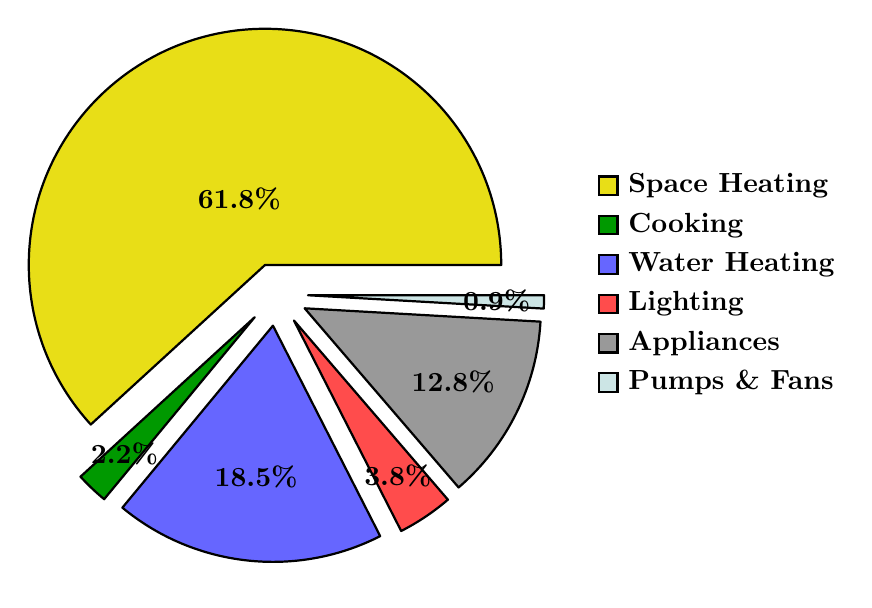
\begin{tikzpicture}
    \tikzstyle{every node}=[font={\bf}]
    \pie[   color = { yellow!90!black, green!60!black, blue!60,
        red!70,
        gray!80,
        teal!20
    }, explode = 0.4, text=legend, radius=3]{61.8/Space Heating, 2.2/Cooking, 18.5/Water Heating, 3.8/Lighting, 12.8/Appliances,0.9/Pumps \& Fans}
    \end{tikzpicture}
    \caption{Ireland 2018 Energy Service Demands}
    \label{fig:Ireland2018ServiceDemands}
\end{figure}

Notably space cooling is absent from Fig \ref{fig:Ireland2018ServiceDemands}, but space cooling is accounted for in appliances. The Policy Oriented Tool for Energy and Climate Change Impact Assessment (POTEnCIA) project disaggregated Ireland's residential space cooling from appliances and have output space cooling energy consumption data, shown in Fig.\ref{fig:Cooling} a significant increase in space cooling energy is expected in the Ireland residential sector. 


\begin{figure}[h]
\centering
\begin{tikzpicture}
\begin{axis}[
    x tick label style={
		/pgf/number format/1000 sep=},xlabel={Year},
	y tick label style={
	    /pgf/number},
		ylabel={Energy Consumption($ktoe$)},
		 scaled y ticks = false,
    xmin=2000, xmax=2050,
    ymin=0, ymax=40,
    xtick={2000,2010,2020,2030,2040,2050},
    ytick={0,10,20,30,40},
    ymajorgrids=true,
]
\addplot[
    color=blue,
    mark=square,
    ]
    coordinates {
    (2000,0.6)(2010,3.1)(2020,8.4)(2030,16.3)(2040,26.1)(2050,37)
    };
\end{axis}
\end{tikzpicture}
    \caption{Space Cooling Residential Energy Consumption (Source: POTEnCIA) }
    \label{fig:Cooling}
\end{figure}

The SEAI residential energy report \cite{SustainableEnergyAuthorityofIreland2018EnergySector} provides high resolution detail on energy demands in the residential sector. Variables such as disposable income, appliance ownership, dwelling location, type of occupier status (owner/rented ), BER label and age of dwelling. 

\subsection{Current Energy Policy}
\label{Intro:Policy}

The energy-related GHG emissions are expected to be reduced beyond the 51\% national target by 2030 compared to 2018, due to the higher cost-effectiveness of abating GHG emissions when compared with agriculture. Despite these high target ambitions in the energy-related GHG emissions, preliminary results from the Environmental Protection Agency (EPA) has indicated a 9\% increase of residential GHG emissions in 2020, mainly due to low home heating oil prices and covid-related restrictions. The CAP2019 Marginal Abatement Cost Curve (MACC), which was developed by McKinsey and Company's modelling tools and is based on EPA's GHG emission projection report \cite{EPA2018EPAReport} found electricity & transport are the most cost effective for decarbonisation \cite{DepartmentofCommunicationsClimateActionandEnvironment2019DecarbonisationIreland}. The future decarbonisation of the residential sector is dependant on receiving low carbon intensity electricity.

Ireland has set out national policy objectives under 10 strategic investment priorities \cite{Ireland2018ProjectFramework}. The first strategic investment priority is ``Compact Growth" which aims to  achieve \textit{``effective density and consolidation, rather than more sprawl of urban development, [as] a top priority"}. Some of these actions included:
\begin{itemize}
    \item{Reducing fossil fuel use in the sector and moving to electricity to provide heating and hot water in buildings}
    \item{500,000 building retrofits to a BER B2 / cost optimal equivalent or carbon equivalent}
    \item{Installation of 600,000 heat pumps, with 400,000 of these in existing buildings}
    \item{Development of district heating, including two initiatives of municipal scale with the potential to provide heat equivalent to the needs of about 50,000 homes}
    \item{Complete the roll-out of the Support Scheme for Renewable Heat}
    \item{Increasing the number of Sustainable Energy Communities to 1,500}
\end{itemize}


\begin{figure}[!htbp]
 \centering
 \includegraphics[scale=1.0]{Figures/CAP2019MACC.png} 
 \caption{Climate Action Plan 2019 - Marginal Abatement Cost Curve}
 \label{fig:CAP2019:MACC} \cite{DepartmentofCommunicationsClimateActionandEnvironment2019Climate2019}
\end{figure}

\par
The CAP2019 MACC, shown in Fig.\ref{fig:CAP2019:MACC} provides $>300$ of the most cost-effective technologies options to reduce Non-ETS GHG by 30\% in 2030 compared to 2005 levels. The x-axis (width of each bar chart) shows the potential reduction of annual $MtCO2_e_q$. The y-axis (height of each bar chart ) shows the associated average cost of abating one tonne of $CO2_e_q$. over the 2021 to 2030 period. The columns are organised from the most economical (left side) to the most expensive technology (right side) in $EUR/tCO2_e_q$ \cite{DepartmentofCommunicationsClimateActionandEnvironment2019Climate2019}. The options specific to the residential sector are: 
\begin{itemize}
    \item{Retrofit oil boiler existing dwellings to B2 equivalent}
    \item{Switch from oil boilers to heat pumps in existing dwellings}
    \item{Retrofit gas boiler and solid fuel stove existing dwellings to B2 equivalent}
    \item{Introduce CO2-free heating in new buildings}\cite{DepartmentofCommunicationsClimateActionandEnvironment2019Climate2019}
\end{itemize} 

Where, the retrofitting of oil boilers is expected to reduce the Total Cost of Ownership (TCO) (ie. save money), but only abate a small amount of carbon, whereas switching oil boilers to heat pumps will increase TCO (ie. cost money) but the expected abatement of carbon is far greater. 


\subsubsection{Electricity}
\par
The decarbonisation of the power generation sector is well underway, with carbon intensity falling annually to 375 $gCO_2/kWh$ in 2018, which is 40\% lower than 2005 levels \cite{Howley2005ENERGY-RELATEDIreland}. Under CAP2019 the continued growth and decarbonisation of the electricity will be the fundamental to lowering energy-related GHG in not only electricity, but in heat and transport also \cite{DepartmentofCommunicationsClimateActionandEnvironment2019Climate2019}.
Decarbonising electricity is key for Ireland, both the \textit{``stick"} (tax) approach which aims to deter investment in fossil fuel power generation, and the \textit{``carrot"} (subsidies) approach which aims to encourage renewable electricity is applied in Irish policy.
In Ireland, a €15/ $tCO_2$ carbon tax was introduced in 2009 to reduce fossil fuel demand and investment. The carbon tax receipts grew every year from 2010 to 2018 \cite{Oireachtas2019AnOffice}. Ireland's current carbon tax of €33.50/ $tCO_2$ will rise to €100/ $tCO_2$ in 2030. Many countries have taken this approach, especially in Europe, where Sweden were second to introduce a carbon tax after Finland, the Swedish carbon tax rate is the highest in the world at €108.81/ $tCO_2$.  About 15\% of global GHG emissions have either an associated cost or tax, this figure is increasing incrementally \cite{WorldBankGroup2020State2020}. 
The Renewable Energy Feed-in Tariff (REFIT) schemes were designed to incentivise Ireland to invest in renewable electricity to achieve legally binding renewable targets under 2009/28/EC. REFIT operates by guaranteeing  new renewable generation and biomass a minimum price for electricity over a 15 year period. The last REFIT schemes closed in December 2015. In 2020 REFIT was replaced by the Renewable Electricity Support Scheme (RESS), which supports to renewable electricity projects to help Ireland achieve 2030 climate targets, especially the 70\% renewable electricity target. RESS delivers for communities to participate in renewable energy projects and increasing technology diversity by broadening the renewable electricity technology mix, where almost 800 MW of solar has been approved in RESS-1 \cite{Eirgrid2020RenewableResults}, this builds alot on the current solar capacity of 16 MW, while making significant progress towards the CAP2019 target of 1500 MW by 2030.

\subsubsection{Heat}
%Gas Network Ireland (GNI) anticipates that by 2026 or 2027 the supply from Corrib ( Irelands only indigenous gas supply, which provided 61\% of gas in 2018 ) will be less than 30\% of 2018 levels \cite{OCleirigh2020ENERGYReport}.
Sustainable Energy Authority of Ireland (SEAI) have been played a leading role in the uptake of building fabric upgrades and heat pumps installations in existing homes. SEAI provide numerous grants to homeowners, increase public awareness of the benefits and are working on simplifying the process. In parallel, new dwellings must achieve a minimum of 20\% renewable energy, the ambient heat used in heat pumps is included as a renewable energy, often heat pumps are the preferred heating technology despite the high capital costs. As mentioned in Section\ref{Intro:IreRSDBack} new buildings in Ireland produce 70\% less GHG emissions than building in 2005 and Section\ref{Intro:Policy} mentioned CAP2019 plans to upgrade 500,000 existing homes to a Building Energy Rating (BER) ‘B2’ by 2030.  The energy efficiency first approach in how Ireland aims to decarbonize the residential sector. Domestic supports for renewable heat or energy efficiency include:
\begin{itemize}
    \item {Insulation}
    \subitem {Attic}
    \subitem {Cavity Wall}
    \subitem {Internal - Dry Lining}
    \subitem {External}
    \item {Heat Pumps}
    \subitem {Air to Water}
    \subitem {Ground Source to Water}
    \subitem {Exhaust Air to Water}
    \subitem {Water to Water}
    \subitem {Air to Air}
    \item {Heating Controls}
    \item {Solar Water Heating}
\end{itemize}

\subsubsection{Gas \& District Heating}

In a bid not to be left behind in a ``net-zero" future, Gas Network Ireland (GNI) have set a 18\% biomethane target for 2030 \cite{Ervia2019AIreland}, where CAP2019 only set a 3\% biomethane target for 2030 \cite{DepartmentofCommunicationsClimateActionandEnvironment2019Climate2019}. GNI plans to met ``net-zero" in 2050 by using 50\% Carbon Capture and Storage (CCS), 37\% biomethane and about 13\% Hydrogen\cite{Ervia2019AIreland}. The gas network currently reaches 40\% or 680,000 dwellings in urban areas, but with the ``Compact Growth" as mentioned in section \ref{Intro:Policy} a higher share of building may have access to the gas network in the future. Increasing biomethane from an agricultural source in the gas network is the most expensive option in CAP2019's MACC shown in Fig.\ref{fig:CAP2019:MACC}. 

Ireland has one of the lowest shares of District Heating (DH) in Europe at less than 1\%  \cite{Gartland2016AIreland} \cite{Harney2020DeterminingIreland}
In Ireland,  DH networks are a new, despite being used for decade across central Europe. CAP2019 plans to have approx. 0.4\% of heating provided by DH in 2030, where the  Research in Ireland h
IrDEA Up to 57\% feasible - same as Denmark DH
37% of the Irish heat demand to district heatingshows that the district heating option provides a solution that ismore efficient than an individual heating solution for 80% 2050 reduction 
potential for 37% district heating nationally (Connollyet al., 2013a).
HVO, solar may also play a part. 

\section{Literature Review}
\label{LitR}

``How should Ireland set GHG targets in the residential sector?” 
Choosing the Pathways which Create the Least Burden
and Offer the Most Opportunity for Ireland
\subsection{Modelling Approach}
\label{LitR:Approach}
\subsection{Supply}
\label{LitR:Supply}
\subsection{Demand}
\label{LitR:Demand}
\subsection{Assumptions}
\label{LitR:Assumptions}
 % LIT REW INPUT DATA - EU \cite{Simoes2013TheProject} 
- LI,er.alThe nationwide survey identified existing technologies, age,
income, region, dwelling characteristics, and knowledge of eco- technology as the six most influential factors for determining homeowners' preferences for heating systems. Among
%the new A-rated houses behave distinctively different which much less demand on space heating and with pumps and fans energy consumption usage increasing, while appliance end use is increasing across the BER ratings. The number of appliances has increased rapidly and while energy efficient improves are  reducing the energy per appliance, it is overshadowed by the growth in electrical appliances. There retrofitting grant which  requires building to have a HLI indication of 2 or less before a heat pump grant can be installs. Ireland’s aim of retrofitting 0.5 million homes from the existing 1.7 million in the before 2030. The effect of these targets also stretches out across the construction sector. The savings from retrofits will decrease fossil fuel energy usage, while most houses 00\% would need to get heat pumps too, to fulfil 0.4 million existing houses getting heat pumps.  This energy efficiency first approach would allow for future technology choices, when current boiler are not at end of life. 

TIM was built to help Ireland provide a pathway to achieve 2030 and 2050 targets. The residential sector plays a key part of this and it was built from the SEAI 2018 energy balance, the BER database and CSO data. The data filtration process used in the residential sector, derived a lot of conversation of the BER database, a group know as Ireland Energy Wiki by the National Retrofitting Modelling Group grew from building the residential sector, questions about the filters, default values, assumptions around thermal equations (EC..) and uncertainties were used to improve the data before it was used in TIM . TIM has many internal project deadines, which required extensive meetings about the data, constraints and results as the modelling was progressing. The data and results were presented to 30 external reviewers to provide feedback, this process proved invaluable having different expertise with different presepectives enabled TIM to fill in gaps. TIM will also be open platform to help improve the model and provide transparency. TIM’s residential sector was built in parallel with LEAP’s residential sector, so that residential sector can easily simulate policy. The demand for results from TIM has increased significantly with increased government ambition, TIM will provide input into CAP 2021 and Ireland’s carbon budgets, working with DECC and the CCAC respectively will also provide feedback and improve the robustness of TIM. for these reasons TIM residential sector is a state of the art modelling platform. 
\section{Results}
\label{Results}
\subsection{Trajectories}
\label{LitR:Traj}
%% The Appendices part is started with the command \appendix;
%% appendix sections are then done as normal sections
\section{Conclusion}
\label{Conclusion}
\section{Discussion}
\label{Discussion}
\section{Acknowledgements}
\label{sec:Acknowledgements}
%CAPACITY is funded under the Climate Action Modelling Group (CAMG) by DECC
% https://www.marei.ie/project/capacity/
CHIMERA is supported by a research grant from Science Foundation Ireland (SFI) and the National Natural Science Foundation of China (NSFC) under the SFI-NSFC Partnership Programme, grant no. 17/NSFC/5181 and
supported by MaREI, the SFI Research Centre for Energy, Climate, and Marine [Grant No: 12/RC/2302\_P2]


https://www.marei.ie/project/chimera/
\appendix

\section{Sample Appendix Section}
\label{sec:sample:appendix}
XXXXXXXX

%% If you have bibdatabase file and want bibtex to generate the
%% bibitems, please use
%%

\printbibliography

%% else use the following coding to input the bibitems directly in the
%% TeX file.

%%\begin{thebibliography}{00}


% %% \bibitem[Author(year)]{label}
% %% Text of bibliographic item

% \bibitem[ ()]{}

% \end{thebibliography}
\end{document}
\endinput
%%
%% End of file `elsarticle-template-harv.tex'.
